\documentclass[11pt]{article}
\usepackage[margin=1in]{geometry}
\usepackage[T1]{fontenc}
\usepackage[utf8]{inputenc}
\usepackage{microtype}
\usepackage{amsmath,amssymb,amsthm,mathtools}
\usepackage{bm}
\usepackage{booktabs,longtable,array}
\usepackage{graphicx}
\usepackage{caption}
\usepackage{subcaption}
\usepackage{enumitem}
\usepackage{xcolor}
\usepackage{hyperref}
\usepackage[nameinlink,capitalize,noabbrev]{cleveref}
\usepackage{url}
\usepackage{listings}
\usepackage{fancyhdr}
\usepackage{setspace}
\hypersetup{colorlinks=true,linkcolor=blue!50!black,citecolor=green!40!black,urlcolor=blue!60!black,
  pdftitle={Noncommutative Cumulant Frontiers for the Fabius--Rvachev Law},
  pdfauthor={OpenAI GPT-5.6 Pro}}
\allowdisplaybreaks
\setlength{\headheight}{14pt}
\emergencystretch=2em
\setstretch{1.04}
\setlength{\parindent}{1.2em}
\setlength{\parskip}{0.15em}
\pagestyle{fancy}
\fancyhf{}
\fancyhead[L]{Fabius--Rvachev cumulant frontiers}
\fancyhead[R]{\thepage}
\renewcommand{\headrulewidth}{0.3pt}
\newtheorem{theorem}{Theorem}[section]
\newtheorem{proposition}[theorem]{Proposition}
\newtheorem{lemma}[theorem]{Lemma}
\newtheorem{corollary}[theorem]{Corollary}
\newtheorem{conjecture}[theorem]{Conjecture}
\newtheorem{problem}[theorem]{Problem}
\theoremstyle{definition}
\newtheorem{definition}[theorem]{Definition}
\newtheorem{remark}[theorem]{Remark}
\newtheorem{experiment}[theorem]{Computational experiment}
\newcommand{\Up}{\operatorname{up}}
\newcommand{\sinc}{\operatorname{sinc}}
\newcommand{\NC}{\mathrm{NC}}
\newcommand{\E}{\mathbb{E}}
\newcommand{\R}{\mathbb{R}}
\newcommand{\Var}{\operatorname{Var}}

\title{\bfseries Noncommutative Cumulant Frontiers for the Fabius--Rvachev Law\\[0.4em]
\large Free and Boolean probability, exact Hankel obstructions, geometric sinc products, Jacobi stripping, and dyadic acceleration}
\author{Research report prepared from the \texttt{ProveIt/Analysis/FabiusFunction/docs} corpus}
\date{30 August 2026}

\begin{document}
\maketitle
\begin{abstract}
The Fabius function and Rvachev's compactly supported \(C^\infty\) function \(\Up\) sit at the meeting point of dyadic functional equations, the Thue--Morse sequence, infinite sinc products, Bernoulli and Bell polynomials, \(q\)-series, orthogonal polynomials, and Lambert--\(W\) endpoint asymptotics. The accompanying repository corpus develops these classical, analytic, arithmetic, and representation-theoretic directions in great depth. This report adds a different layer: free and Boolean cumulants of the probability law with density \(\Up\), together with their interaction with the existing Jacobi, \(q\)-binomial, finite-sinc, inverse-Fabius, Legendre, and endpoint frameworks.

The main proved result is an exact rational certificate that the Rvachev up-law is \emph{not} freely infinitely divisible. After variance normalization, a \(3\times3\) shifted free-cumulant Hankel block has negative determinant; an even simpler polynomial test vector gives a negative quadratic form. We extend this obstruction to the geometric-uniform family
\[
Y_q=\sum_{k\ge1}q^kU_k,\qquad U_k\stackrel{\mathrm{iid}}\sim \mathrm{Unif}[-1,1],
\]
proving non-free-infinite-divisibility for every \(0<q<0.523498599534498\ldots\), including \(q=1/2\). The endpoint is the square root of a rigorously isolated root of an explicit degree-thirty integer polynomial.

Further exact bridges are obtained. Lagrange inversion turns the Bernoulli--Bell moment formula into a finite formula for free cumulants. Boolean cumulants are identified with moments of the once-stripped Jacobi measure, proving strict positivity. Every fixed-order free or Boolean cumulant of a finite dyadic sinc product is an exact polynomial in \(4^{-N}\), so the repository's \(q=1/4\) Richardson and \(q\)-binomial acceleration machinery applies directly. A Legendre-coefficient transform and an inverse-Fabius integral transform are given explicitly. Finally, symbolic evidence through \(r_{16}\), exact positivity through \(r_{120}\), and endpoint computations motivate conjectures on Jacobi increments, free-cumulant positivity, and a Lambert--\(W\)-controlled transform radius.
\end{abstract}

\noindent\textbf{Status convention.}
Statements labelled theorem, proposition, lemma, or corollary are proved. Statements labelled computational experiment are exact or high-precision calculations reproducible by the included Python program. Conjectures and problems are explicitly marked.

\tableofcontents
\newpage

\section{Corpus audit, novelty screen, and scope}
\subsection{The audited documentation tree}
The requested source tree is not a single article but a layered research corpus. Its live top level contains a mathematical glossary, the principal Fabius--Rvachev exposition, a non-elementarity study, a Lean walkthrough, an archive, a paper collection, and both semi-formalized and non-formalized frontier branches. The semi-formalized branch further records a canonical consolidated source, a proof-dependency manifest, a gap register, and many thematic drafts.

The frontier manifest is especially important for a novelty audit. It states that eleven earlier notebooks were consolidated into six main syntheses and a gap register, and it records provenance for work on dyadic formulae, \(q\)-connections, small-argument and endpoint asymptotics, repeated integration, inverse-function saddles, and Thue--Morse convergence. It also lists later large volumes devoted to representations, exponents and \(q\)-series, polynomial synthesis, dyadic combs and finite sinc products, all-orders inverse endpoint asymptotics, Lambert--\(W\), and a broad \(q\)-Pochhammer/\(q\)-binomial monograph.

Consequently, several apparently natural directions are not new relative to the repository. A report centered only on Jacobi coefficients, Legendre expansions, Mellin transforms, Pad\'e approximation, finite sinc products, Richardson extrapolation, or Lambert--\(W\) endpoint inversion would duplicate substantial existing material. The present report uses those results as interfaces and develops a noncommutative cumulant layer not found in the audited sources.

\subsection{New contributions}
The main additions are:
\begin{enumerate}[label=\textbf{N\arabic*.},leftmargin=3.2em]
\item an exact free-cumulant transform of the Bernoulli--Bell moment formulas;
\item an exact proof that the dyadic up-law is not freely infinitely divisible;
\item a parameter-uniform obstruction for \(0<q<0.5234985995\ldots\);
\item a Boolean-cumulant coefficient-stripping theorem for the Jacobi continued fraction;
\item exact \(4^{-N}\)-polynomial laws for free and Boolean cumulants of finite dyadic sinc products;
\item inverse-Fabius and finite Legendre transforms for these cumulants;
\item a Jacobi-increment positivity conjecture verified through \(r_{16}\);
\item endpoint conjectures connecting Lambert--\(W\) flatness to transform radii.
\end{enumerate}
The novelty claim is relative to the repository corpus. Free and Boolean cumulants and their general relations to Jacobi parameters are established topics; the new content is their specialization to the Fabius--Rvachev law, the exact rational and \(q\)-parametric certificates, and the bridges to the existing dyadic machinery.

\subsection{Notation and normalization}
Write \(U\sim\mathrm{Unif}[-1,1]\), so
\[
\E e^{tU}=\frac{\sinh t}{t},\qquad \E e^{itU}=\sinc t:=\frac{\sin t}{t}.
\]
Let \(U_1,U_2,\ldots\) be independent copies. For \(0<q<1\), define
\begin{equation}\label{eq:Yq}
Y_q:=\sum_{k=1}^{\infty}q^kU_k.
\end{equation}
Its support is \([-q/(1-q),q/(1-q)]\). At \(q=1/2\), the support is \([-1,1]\), and the density is Rvachev's \(\Up\) function normalized by \(\int_{-1}^1\Up(x)\,dx=1\). The law for negative \(q\) is the same as for \(|q|\), because the summands are symmetric.

The repository also uses a unit-support geometric normalization with weights \((1-q)q^k\). It differs only by a nonzero scalar. Free infinite divisibility and variance-normalized cumulants are invariant under scaling, so \eqref{eq:Yq} is algebraically convenient.

\section{Classical dyadic structure as probabilistic input}
\subsection{Infinite sinc products and the Rvachev law}
Independence gives
\begin{align}
\phi_q(t)&:=\E e^{itY_q}=\prod_{k=1}^{\infty}\sinc(q^kt),\label{eq:charprod}\\
\mathcal M_q(t)&:=\E e^{tY_q}=\prod_{k=1}^{\infty}\frac{\sinh(q^kt)}{q^kt}.\label{eq:mgfprod}
\end{align}
For \(q=1/2\), \eqref{eq:charprod} is the standard infinite sinc product for \(\Up\). The random series gives the fixed point
\begin{equation}\label{eq:fixedY}
Y_{1/2}\stackrel{d}{=}\frac{Y_{1/2}'+U}{2},
\end{equation}
where \(Y_{1/2}'\) is an independent copy.

\subsection{Bernoulli cumulants}
Use the convention \(B_2=1/6\), \(B_4=-1/30\). Since
\[
\log\frac{\sinh t}{t}=\sum_{m\ge1}\frac{2^{2m}B_{2m}}{2m}\frac{t^{2m}}{(2m)!},
\]
classical cumulants add and scale to give the following.

\begin{proposition}[Classical cumulants]\label{prop:classicalq}
For \(m\ge1\),
\begin{equation}\label{eq:kappaq}
\kappa_{2m}(Y_q)=\frac{2^{2m}B_{2m}}{2m}\frac{q^{2m}}{1-q^{2m}},
\qquad \kappa_{2m+1}(Y_q)=0.
\end{equation}
At \(q=1/2\),
\begin{equation}\label{eq:kappadyadic}
\kappa_{2m}=\frac{4^mB_{2m}}{2m(4^m-1)}.
\end{equation}
\end{proposition}
\begin{proof}
Apply the uniform cumulant expansion to each \(q^kU_k\), then sum \(\sum_{k\ge1}q^{2mk}=q^{2m}/(1-q^{2m})\).
\end{proof}

Let \(m_n=\E Y^n\). The complete exponential Bell polynomial gives
\begin{equation}\label{eq:bellmoment}
m_n=B_n(\kappa_1,\ldots,\kappa_n),
\end{equation}
and equivalently
\begin{equation}\label{eq:momentcumrec}
m_n=\sum_{j=1}^n\binom{n-1}{j-1}\kappa_jm_{n-j},\qquad m_0=1.
\end{equation}

\subsection{A positive dyadic moment recurrence}
\begin{proposition}[Stable dyadic moment recurrence]\label{prop:momentrec}
For \(m_{2n}=\E Y_{1/2}^{2n}\),
\begin{equation}\label{eq:dyadicmomentrec}
(4^n-1)m_{2n}=\sum_{k=1}^n\binom{2n}{2k}\frac{m_{2n-2k}}{2k+1},\qquad m_0=1.
\end{equation}
\end{proposition}
\begin{proof}
Raise \eqref{eq:fixedY} to power \(2n\), expand, and use symmetry. The \(k=0\) term is \(4^{-n}m_{2n}\), and \(\E U^{2k}=1/(2k+1)\).
\end{proof}

\section{Free and Boolean transforms of the moment sequence}
\subsection{Partition cumulants}
Let
\[
M(z)=1+\sum_{n\ge1}m_nz^n.
\]
The free cumulants \(r_n\) are defined by
\begin{equation}\label{eq:NCmoment}
m_n=\sum_{\pi\in\mathrm{NC}(n)}\prod_{V\in\pi}r_{|V|}.
\end{equation}
Equivalently, if \(C(w)=1+\sum_{n\ge1}r_nw^n\), then
\begin{equation}\label{eq:MCrelation}
M(z)=C(zM(z)).
\end{equation}
The Boolean cumulants \(b_n\), associated with interval partitions, satisfy
\begin{equation}\label{eq:booleanrelation}
M(z)=\frac{1}{1-B(z)},\qquad B(z)=\sum_{n\ge1}b_nz^n.
\end{equation}

For a symmetric law, write
\begin{equation}\label{eq:Adef}
A(t):=\sum_{n\ge0}m_{2n}t^n,
\quad D(w):=1+\sum_{n\ge1}r_{2n}w^n,
\quad H(t):=\sum_{n\ge1}b_{2n}t^n.
\end{equation}
Then
\begin{equation}\label{eq:compressedrelations}
A(t)=D\bigl(tA(t)^2\bigr),
\qquad H(t)=1-\frac1{A(t)}.
\end{equation}

\subsection{Lagrange inversion}
\begin{theorem}[Lagrange formula for free cumulants]\label{thm:lagrangefree}
For any moment sequence with \(m_0=1\),
\begin{equation}\label{eq:lagrangegeneral}
r_n=-\frac1{n-1}[z^n]M(z)^{1-n},\qquad n\ge2.
\end{equation}
For a symmetric sequence,
\begin{equation}\label{eq:lagrangesymmetric}
r_{2n}=-\frac1{2n-1}[t^n]A(t)^{1-2n}.
\end{equation}
\end{theorem}
\begin{proof}
Set \(w=zM(z)\), and let \(z=z(w)\) be its compositional inverse. By \eqref{eq:MCrelation}, \(C(w)=M(z(w))\). Lagrange--B\"urmann inversion gives
\[
[w^n]C(w)=\frac1n[z^{n-1}]M'(z)M(z)^{-n}.
\]
Since \((M^{1-n})'=(1-n)M^{-n}M'\), coefficient extraction yields \eqref{eq:lagrangegeneral}. Symmetry gives \(M(z)=A(z^2)\), hence \eqref{eq:lagrangesymmetric}.
\end{proof}

Expanding \((1+X)^{1-2n}\) gives a completely finite formula.
\begin{corollary}[Finite composition formula]\label{cor:compositionfree}
For \(n\ge1\),
\begin{equation}\label{eq:freecomposition}
r_{2n}=\frac1{2n-1}\sum_{k=1}^n(-1)^{k+1}
\binom{2n+k-2}{k}
\sum_{\substack{j_1+\cdots+j_k=n\\j_i\ge1}}
\prod_{i=1}^k m_{2j_i}.
\end{equation}
The Boolean analogue is
\begin{equation}\label{eq:booleancomposition}
b_{2n}=\sum_{k=1}^n(-1)^{k+1}
\sum_{\substack{j_1+\cdots+j_k=n\\j_i\ge1}}
\prod_{i=1}^k m_{2j_i}.
\end{equation}
\end{corollary}

Combining \eqref{eq:kappaq}, \eqref{eq:bellmoment}, and \eqref{eq:freecomposition} is an explicit Bernoulli--Bell--noncrossing transform. It converts the classical Bernoulli cumulants of the infinite sinc product into free cumulants without integration or numerical inversion.

\subsection{Triangular recurrences}
From \eqref{eq:compressedrelations},
\begin{align}
A(t)&=1+\sum_{j\ge1}r_{2j}t^jA(t)^{2j},\label{eq:freerecgen}\\
b_{2n}&=m_{2n}-\sum_{j=1}^{n-1}b_{2j}m_{2n-2j}.
\label{eq:booleanrec}
\end{align}
Thus
\begin{equation}\label{eq:freerec}
r_{2n}=m_{2n}-\sum_{j=1}^{n-1}r_{2j}[t^{n-j}]A(t)^{2j}.
\end{equation}
These recurrences are the basis of the exact rational computations in the accompanying program.

\subsection{First exact dyadic values}
\begin{table}[ht]
\centering
\caption{First even moments, free cumulants, and Boolean cumulants of the dyadic up-law.}
\label{tab:firstcumulants}
\resizebox{\textwidth}{!}{%
\begin{tabular}{c@{\qquad}c@{\qquad}c@{\qquad}c}
\toprule
order & \(m_{2n}\) & \(r_{2n}\) & \(b_{2n}\)\\
\midrule
2 & \(1/9\) & \(1/9\) & \(1/9\)\\
4 & \(19/675\) & \(7/2025\) & \(32/2025\)\\
6 & \(583/59535\) & \(562/893025\) & \(4384/893025\)\\
8 & \(132809/32531625\) & \(55603/379535625\) & \(6845728/3415820625\)\\
10 & \(46840699/24405225075\) & \(148564406/3294705385125\) & \(109557322976/115314688479375\)\\
12 & \(4068990560161/4133856862760625\) & \(3386539245383834/214857210441983484375\) & \(106674881656252384/214857210441983484375\)\\
\bottomrule
\end{tabular}%
}
\end{table}

\begin{experiment}[Exact positivity check]\label{exp:freepositive}
The program computed \(r_{2n}\) by rational arithmetic for \(1\le n\le60\), and every value was positive. Thus positivity is verified exactly through \(r_{120}\), not merely numerically.
\end{experiment}

\section{An exact obstruction to free infinite divisibility}
\subsection{Conditional positive definiteness}
For a compactly supported probability measure, free infinite divisibility implies conditional positive definiteness of its free-cumulant sequence. In one variable, a necessary condition is
\begin{equation}\label{eq:CPD}
\sum_{i,j\ge1}\overline{a_i}a_jr_{i+j}\ge0
\end{equation}
for every finitely supported sequence \((a_i)_{i\ge1}\). Equivalently, every finite principal or nonprincipal submatrix of the shifted Hankel matrix
\[
\mathcal H_r=(r_{i+j})_{i,j\ge1}
\]
must be positive semidefinite. For a symmetric law, odd free cumulants vanish, so this matrix separates into odd- and even-index parity blocks.

\subsection{The dyadic certificate}
\begin{theorem}[The Rvachev up-law is not freely infinitely divisible]\label{thm:upnotFID}
Let \(Y=Y_{1/2}\), and let \(X=3Y\), so \(\Var(X)=1\). Write
\[
c_{2n}:=r_{2n}(X)=3^{2n}r_{2n}(Y).
\]
Then the shifted even block
\begin{equation}\label{eq:Hmatrix}
H=\begin{pmatrix}
c_4&c_6&c_8\\
c_6&c_8&c_{10}\\
c_8&c_{10}&c_{12}
\end{pmatrix}
\end{equation}
has negative determinant. Hence neither \(X\) nor \(Y\) is freely infinitely divisible.
\end{theorem}

\begin{proof}
The exact normalized free cumulants are
\begin{align*}
c_2&=1,& c_4&=\frac7{25},& c_6&=\frac{562}{1225},\\
c_8&=\frac{500427}{520625},&
c_{10}&=\frac{148564406}{55796125},&
c_{12}&=\frac{3386539245383834}{404291747234375}.
\end{align*}
Direct rational elimination gives
\begin{equation}\label{eq:negativeDet}
\det H=-\frac{110020031172003013633803653}
{3288379747918347944189453125}<0.
\end{equation}
Therefore \(H\) is not positive semidefinite, contradicting the necessary condition \eqref{eq:CPD}. Scaling by a nonzero constant preserves free infinite divisibility, so the conclusion holds for \(Y\) as well.
\end{proof}

A shorter certificate avoids a determinant.
\begin{corollary}[Polynomial witness]\label{cor:polywitness}
For \(v=(3,-4,1)^\top\),
\begin{equation}\label{eq:negativeQ}
v^\top Hv=-\frac{108624693817191}{404291747234375}<0.
\end{equation}
Equivalently, the conditional cumulant functional is negative on
\[
p(x)=3x^2-4x^4+x^6=x^2(x^2-1)(x^2-3).
\]
\end{corollary}

\begin{remark}[Positivity is not enough]
The first sixty even free cumulants are positive, yet the shifted Hankel form is indefinite. This cleanly separates coefficientwise positivity from the much stronger conditional positive definiteness required by free infinite divisibility.
\end{remark}

\subsection{A three-way divisibility comparison}
The up-law is nondegenerate and compactly supported, so it is not classically infinitely divisible: a nondegenerate classically infinitely divisible law cannot have bounded support. Theorem~\ref{thm:upnotFID} shows it is not freely infinitely divisible either. In contrast, every probability measure is Boolean infinitely divisible, because Boolean convolution powers are defined by scalar multiplication of the Boolean cumulant series. Thus the up-law gives a concrete trichotomy:
\[
\text{classical ID: no},\qquad \text{free ID: no},\qquad \text{Boolean ID: yes}.
\]

\section{A geometric \texorpdfstring{\(q\)}{q}-family obstruction}
\subsection{Variance-normalized free cumulants}
Put \(s=q^2\) and normalize \(Y_q\) to variance one. Since
\[
\kappa_2(Y_q)=\frac{s}{3(1-s)},
\]
define
\[
c_{2n}(s):=\frac{r_{2n}(Y_q)}{r_2(Y_q)^n}.
\]
These quantities depend only on \(s\), as expected from symmetry and scale invariance.

\begin{proposition}[First normalized free cumulants]\label{prop:qfree}
For \(0<s<1\),
\begin{align}
c_2(s)&=1,\label{eq:c2s}\\
c_4(s)&=\frac{11s-1}{5(1+s)},\label{eq:c4s}\\
c_6(s)&=\frac{2(379s^3+20s^2+20s+1)}{35(1+s)(1+s+s^2)},\label{eq:c6s}\\
c_8(s)&=\frac{3P_8(s)}{175(1+s)^2(1+s^2)(1+s+s^2)},\label{eq:c8s}\\
P_8(s)&=24359s^6+4221s^5+4579s^4+4242s^3+379s^2+21s-1.\nonumber
\end{align}
The formulas for \(c_{10}\) and \(c_{12}\) are given in Appendix~\ref{app:qformulas}.
\end{proposition}
\begin{proof}
Insert \eqref{eq:kappaq} into the Bell recurrence \eqref{eq:momentcumrec}, apply the triangular free recurrence \eqref{eq:freerec}, and divide by \(r_2^n\). Every operation is rational in \(s\), so the displayed identities reduce to polynomial verification.
\end{proof}

The first obstruction is immediate: \(c_4(s)<0\) for \(0<s<1/11\). For larger \(s\), a higher shifted-Hankel block is required.

\subsection{The degree-thirty determinant}
Define
\begin{equation}\label{eq:D3def}
D_3(s):=\det\begin{pmatrix}
c_4(s)&c_6(s)&c_8(s)\\
c_6(s)&c_8(s)&c_{10}(s)\\
c_8(s)&c_{10}(s)&c_{12}(s)
\end{pmatrix}.
\end{equation}
Exact simplification gives
\begin{equation}\label{eq:D3rational}
D_3(s)=\frac{P_{30}(s)}{
11802415625(1+s)^6(1+s^2)^3(1-s+s^2)(1+s+s^2)^4(1+s+s^2+s^3+s^4)^2},
\end{equation}
where \(P_{30}\in\mathbb Z[s]\) is listed in Appendix~\ref{app:P30}. The denominator is positive on \((0,1)\).

Let \(\alpha\) be the largest positive root of \(P_{30}\). Exact Sturm-sequence computations isolate it in
\begin{equation}\label{eq:alphainterval}
\frac{385546279}{1406842461}<\alpha<\frac{219810848}{802080713}
\end{equation}
and give
\begin{equation}\label{eq:alphaapprox}
\alpha=0.274050783714581103197636083256401808258849748968\ldots.
\end{equation}
The same Sturm certificate shows that there are no roots of \(P_{30}\) in \((1/11,\alpha)\). Since \(D_3(1/4)<0\), it follows that \(D_3(s)<0\) throughout that interval.

\begin{theorem}[Geometric non-free-infinite-divisibility interval]\label{thm:qnotFID}
Let \(Y_q\) be defined by \eqref{eq:Yq}. If
\begin{equation}\label{eq:qthreshold}
0<q<\sqrt\alpha
=0.52349859953449837591\ldots,
\end{equation}
then \(Y_q\) is not freely infinitely divisible.
\end{theorem}
\begin{proof}
If \(0<s<1/11\), then \(c_4(s)<0\), violating conditional positive definiteness. If \(1/11\le s<\alpha\), then \(D_3(s)<0\), so the block in \eqref{eq:D3def} is not positive semidefinite. Since \(s=q^2\), the stated range follows.
\end{proof}

\begin{remark}
The dyadic point \(q=1/2\) has \(s=1/4<\alpha\), so Theorem~\ref{thm:upnotFID} is recovered. The direct rational certificate of Section~4 is nevertheless preferable at the dyadic point because it is shorter and does not invoke root isolation.
\end{remark}

\subsection{A hierarchy of necessary-condition thresholds}
For each \(m\ge1\), form the leading \(m\times m\) even shifted-Hankel block
\[
H_m(s)=\bigl(c_{2(i+j)}(s)\bigr)_{1\le i,j\le m}.
\]
The following are the largest zeros detected numerically for \(\det H_m(s)\) in the searched interval.

\begin{table}[ht]
\centering
\caption{Numerical leading-block thresholds. These are necessary-condition diagnostics, not a proof of free infinite divisibility above the listed values.}
\label{tab:hankelthresholds}
\begin{tabular}{rcc}
\toprule
\(m\) & largest detected \(s\)-zero & \(q=\sqrt{s}\)\\
\midrule
1 & 0.090909090909090909 & 0.301511344577764\\
2 & 0.199485938552759446 & 0.446638487540829\\
3 & 0.274050783714581103 & 0.523498599534498\\
4 & 0.320508711922987676 & 0.566134888452379\\
5 & 0.349023432785722262 & 0.590782051847991\\
6 & 0.366350957768133855 & 0.605269326637435\\
7 & 0.376359680090712126 & 0.613481605340137\\
8 & 0.381275825505797916 & 0.617475364290591\\
9 & 0.382775958248985252 & 0.618688902639271\\
10& 0.382808454300472788 & 0.618715164110653\\
\bottomrule
\end{tabular}
\end{table}

\begin{figure}[ht]
\centering
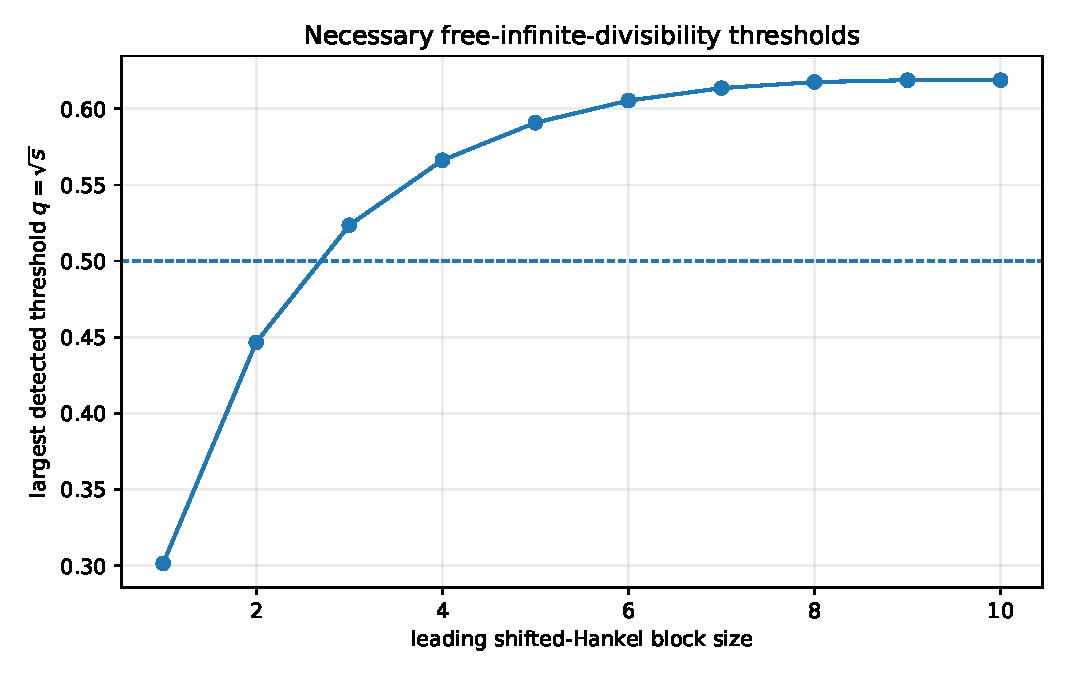
\includegraphics[width=0.76\textwidth]{figures/hankel_thresholds.pdf}
\caption{Largest detected zero of the leading even shifted-Hankel determinant. The dashed line marks the dyadic parameter \(q=1/2\).}
\label{fig:hankelthresholds}
\end{figure}

\begin{problem}[Free-divisibility phase diagram]\label{prob:phase}
Determine the set
\[
\mathcal F:=\{q\in(0,1):Y_q\text{ is freely infinitely divisible}\}.
\]
The present work proves \(\mathcal F\cap(0,\sqrt\alpha)=\varnothing\). Two plausible scenarios remain: a genuine threshold after which all laws are freely infinitely divisible, or failure for every finite \(q<1\) with free infinite divisibility appearing only in the Gaussian limit.
\end{problem}

\subsection{The Gaussian endpoint and connected partitions}
Let \(Z_q=Y_q/\sqrt{\Var(Y_q)}\). From \eqref{eq:kappaq}, the standardized classical cumulants satisfy
\begin{equation}\label{eq:stdclassical}
\lambda_{2m}(s)=
\frac{3^m2^{2m}B_{2m}}{2m}\frac{(1-s)^m}{1-s^m},
\end{equation}
so \(\lambda_2=1\) and \(\lambda_{2m}=O((1-s)^{m-1})\) for \(m\ge2\). Thus \(Z_q\) converges in moments and distribution to the standard normal law as \(q\uparrow1\).

The free cumulants of the standard normal enumerate connected pairings. Consequently,
\begin{equation}\label{eq:normalfree}
(c_2,c_4,c_6,c_8,c_{10},c_{12})\longrightarrow(1,1,4,27,248,2830).
\end{equation}
Writing \(\varepsilon=1-s\), exact expansion of Proposition~\ref{prop:qfree} and Appendix~\ref{app:qformulas} gives
\begin{align}
c_4&=1-\frac35\varepsilon+O(\varepsilon^2),\nonumber\\
c_6&=4-\frac{27}{5}\varepsilon+O(\varepsilon^2),\nonumber\\
c_8&=27-\frac{306}{5}\varepsilon+O(\varepsilon^2),\label{eq:gausscorrections}\\
c_{10}&=248-831\varepsilon+O(\varepsilon^2),\nonumber\\
c_{12}&=2830-\frac{65178}{5}\varepsilon+O(\varepsilon^2).\nonumber
\end{align}
Only \(\lambda_4=-(3/5)\varepsilon+O(\varepsilon^2)\) contributes at first order. Lehner's connected-partition formula therefore gives an enumerative interpretation.

\begin{proposition}[First Gaussian correction]\label{prop:connectedcorrection}
Let \(A_n\) be the number of connected set partitions of \([2n]\), in Lehner's sense, with one block of size four and all remaining blocks of size two. Then
\begin{equation}\label{eq:connectedcorrection}
c_{2n}(s)=\gamma_n-\frac35A_n(1-s)+O((1-s)^2),
\end{equation}
where \(\gamma_n\) is the number of connected pairings of \([2n]\). For \(n=2,\ldots,6\),
\[
A_n=1,9,102,1385,21726.
\]
\end{proposition}
\begin{proof}
Free cumulants are sums over connected set partitions weighted by classical cumulants. At \(s=1\), only \(\lambda_2=1\) survives, giving connected pairings. To first order in \(1-s\), exactly one block may carry \(\lambda_4=-(3/5)(1-s)+O((1-s)^2)\); all other blocks are pairs. Higher classical cumulants contribute only at second or higher order.
\end{proof}

\section{Boolean cumulants and Jacobi coefficient stripping}
\subsection{The Stieltjes continued fraction}
The repository develops the symmetric Jacobi matrix and the Stieltjes continued fraction of the even moment series. Write
\begin{equation}\label{eq:Sfraction}
A(t)=
\cfrac{1}{1-\cfrac{\beta_1t}{1-\cfrac{\beta_2t}{1-\cfrac{\beta_3t}{\ddots}}}},
\qquad \beta_j>0.
\end{equation}
For the up-law, the first coefficients include
\begin{equation}\label{eq:firstbetas}
\beta_1=\frac19,
\qquad
\beta_2=\frac{32}{225}.
\end{equation}
The associated Jacobi operator has zero diagonal, because the measure is symmetric.

\begin{theorem}[Boolean coefficient stripping]\label{thm:booleanstrip}
Let \(A\) have the S-fraction \eqref{eq:Sfraction}, and let
\[
A^{(1)}(t)=
\cfrac{1}{1-\cfrac{\beta_2t}{1-\cfrac{\beta_3t}{\ddots}}}
\]
be the once-stripped tail. Then
\begin{equation}\label{eq:booleanstrip}
H(t)=1-\frac1{A(t)}=\beta_1tA^{(1)}(t).
\end{equation}
Consequently,
\begin{equation}\label{eq:booleanassociated}
b_{2n}=\beta_1m_{n-1}^{(1)}>0,
\end{equation}
where \(m_k^{(1)}=[t^k]A^{(1)}(t)\) is the \(k\)th moment of the first associated Jacobi measure.
\end{theorem}
\begin{proof}
Remove the first denominator in \eqref{eq:Sfraction}:
\[
A(t)=\frac1{1-\beta_1tA^{(1)}(t)}.
\]
Substitution into \(H=1-A^{-1}\) proves \eqref{eq:booleanstrip}. Since \(\beta_j>0\), the tail is a Stieltjes moment series with positive coefficients; the up-law has infinite support, so the coefficients are strictly positive.
\end{proof}

\begin{remark}
This identifies Boolean cumulants not merely as recursively defined rational numbers but as a shifted moment sequence of an associated orthogonality measure. It creates a direct bridge between noncommutative probability and the repository's Jacobi/Legendre representation program.
\end{remark}

\subsection{Jacobi increments and free-cumulant positivity}
Let
\begin{equation}\label{eq:deltabeta}
\Delta_j:=\beta_{j+1}-\beta_j.
\end{equation}
The first free cumulants, re-expanded in \(\beta_1\) and the increments, are
\begin{align}
r_2&=\beta_1,\label{eq:r2beta}\\
r_4&=\beta_1\Delta_1,\label{eq:r4beta}\\
r_6&=\beta_1\bigl(2\Delta_1^2+\beta_2\Delta_2\bigr),\label{eq:r6beta}\\
r_8&=\beta_1\bigl(
\beta_1^2\Delta_3+6\beta_1\Delta_1\Delta_2
+2\beta_1\Delta_1\Delta_3+2\beta_1\Delta_2^2
+\beta_1\Delta_2\Delta_3\nonumber\\
&\hspace{7em}+5\Delta_1^3+6\Delta_1^2\Delta_2
+\Delta_1^2\Delta_3+2\Delta_1\Delta_2^2
+\Delta_1\Delta_2\Delta_3\bigr).
\label{eq:r8beta}
\end{align}
These formulas were obtained by expanding the weighted-Dyck-path moments of \eqref{eq:Sfraction}, applying \eqref{eq:freerec}, and substituting \(\beta_j=\beta_1+\Delta_1+\cdots+\Delta_{j-1}\).

\begin{experiment}[Jacobi-increment positivity through \(r_{16}\)]\label{exp:jacobiincrements}
The exact symbolic expansion has nonnegative integer coefficients at every checked order. The monomial counts are
\begin{center}
\begin{tabular}{c|rrrrrrr}
\toprule
cumulant & \(r_4\)&\(r_6\)&\(r_8\)&\(r_{10}\)&\(r_{12}\)&\(r_{14}\)&\(r_{16}\)\\
\midrule
monomials &1&3&10&35&120&410&1400\\
\bottomrule
\end{tabular}
\end{center}
All coefficients were checked exactly as integers.
\end{experiment}

\begin{conjecture}[Jacobi-increment positivity]\label{conj:jacobiincrements}
For every \(n\ge1\), \(r_{2n}/\beta_1\) is a polynomial with nonnegative integer coefficients in
\[
\beta_1,\Delta_1,\ldots,\Delta_{n-1}.
\]
Therefore any symmetric measure with nondecreasing S-fraction coefficients \(\beta_j\) has nonnegative even free cumulants.
\end{conjecture}

A proof would likely require a sign-free reinterpretation of Lehner's lattice-path formula after coefficient stripping. The repository conjectures monotone behavior of the up-law's Jacobi coefficients toward the arcsine limit \(1/4\); Conjecture~\ref{conj:jacobiincrements} would convert such monotonicity into free-cumulant positivity. Theorem~\ref{thm:upnotFID} shows that this still would not imply free infinite divisibility.

\section{Interfaces with inverse Fabius and Legendre expansions}
\subsection{An inverse-Fabius moment identity}
On \([0,1]\), the standard relation between the two functions is
\begin{equation}\label{eq:upF}
\Up(x)=F(1-x),
\end{equation}
with \(\Up\) even. Therefore
\begin{equation}\label{eq:momentF}
m_{2n}=2\int_0^1x^{2n}F(1-x)\,dx
      =2\int_0^1(1-y)^{2n}F(y)\,dy.
\end{equation}
Integration by parts and the substitution \(u=F(y)\) give a useful inverse-function formula.

\begin{proposition}[Inverse-Fabius representation]\label{prop:inverseFmoment}
For \(n\ge0\),
\begin{equation}\label{eq:inverseFmoment}
m_{2n}=\frac{2}{2n+1}\int_0^1\bigl(1-F^{-1}(u)\bigr)^{2n+1}\,du.
\end{equation}
\end{proposition}
\begin{proof}
In the last integral of \eqref{eq:momentF}, integrate \((1-y)^{2n}\) and differentiate \(F(y)\). The boundary terms vanish because \(F(0)=0\) and \((1-y)^{2n+1}=0\) at \(y=1\). Thus
\[
m_{2n}=\frac{2}{2n+1}\int_0^1(1-y)^{2n+1}F'(y)\,dy.
\]
Now set \(u=F(y)\).
\end{proof}

Combining \eqref{eq:inverseFmoment} with Theorem~\ref{thm:lagrangefree} gives an explicit inverse-Fabius/free-cumulant bridge:
\begin{equation}\label{eq:inverseFfree}
r_{2n}=-\frac1{2n-1}[t^n]
\left(
1+\sum_{j\ge1}\frac{2t^j}{2j+1}
\int_0^1(1-F^{-1}(u))^{2j+1}\,du
\right)^{1-2n}.
\end{equation}
The corresponding Boolean formula is obtained by replacing the outer power with \(1-(\cdot)^{-1}\). Thus every free or Boolean cumulant is a finite polynomial in integral moments of the inverse Fabius function.

\subsection{A finite transform from Legendre coefficients}
Suppose the even Legendre expansion is
\begin{equation}\label{eq:Legendreseries}
\Up(x)=\sum_{k\ge0}a_{2k}P_{2k}(x),
\end{equation}
with the repository's normalization of \(P_n\). Orthogonality is not needed for the following triangular transform; only the standard integral
\begin{equation}\label{eq:xPintegral}
\int_{-1}^1x^{2n}P_{2k}(x)\,dx
=\frac{2(2n)!}{(2n-2k)!!(2n+2k+1)!!},
\qquad 0\le k\le n.
\end{equation}

\begin{proposition}[Legendre-to-cumulant transform]\label{prop:Legendretransform}
The moment \(m_{2n}\) depends only on \(a_0,a_2,\ldots,a_{2n}\), namely
\begin{equation}\label{eq:Legendremoment}
m_{2n}=\sum_{k=0}^n
\frac{2(2n)!}{(2n-2k)!!(2n+2k+1)!!}\,a_{2k}.
\end{equation}
Consequently, \(r_{2n}\) and \(b_{2n}\) are finite polynomial functions of the first \(n+1\) even Legendre coefficients.
\end{proposition}
\begin{proof}
Insert \eqref{eq:Legendreseries} into \(m_{2n}=\int_{-1}^1x^{2n}\Up(x)\,dx\). Terms with \(k>n\) vanish, and \eqref{eq:xPintegral} yields \eqref{eq:Legendremoment}. Apply \eqref{eq:freecomposition} and \eqref{eq:booleancomposition}.
\end{proof}

This is useful computationally in both directions. High-quality Legendre coefficients produce free and Boolean cumulants without sampling \(\Up\); conversely, exact cumulants supply nonlinear consistency checks on numerically computed Legendre expansions.

\section{Finite dyadic sinc products and exact \texorpdfstring{\(q=1/4\)}{q=1/4} acceleration}
\subsection{Partial random series}
Define the finite dyadic approximation
\begin{equation}\label{eq:finiteY}
Y^{(N)}:=\sum_{k=1}^N2^{-k}U_k,
\qquad Q:=4^{-N}.
\end{equation}
Its characteristic function is the finite sinc product
\[
\phi_N(t)=\prod_{k=1}^N\sinc(t/2^k),
\]
and its density is a compactly supported spline whose signed knot structure is governed by dyadic subset sums and the Thue--Morse parity pattern. The classical cumulants truncate geometrically:
\begin{equation}\label{eq:finiteclassical}
\kappa_{2m}^{(N)}=\kappa_{2m}(1-Q^m).
\end{equation}

\begin{theorem}[Polynomial transfer law]\label{thm:finitepolynomial}
Fix \(n\ge1\). Each of the quantities
\[
m_{2n}^{(N)},\qquad r_{2n}^{(N)},\qquad b_{2n}^{(N)}
\]
is an exact polynomial in \(Q=4^{-N}\) of degree at most \(n\). Its constant term is the corresponding cumulant or moment of the infinite up-law.
\end{theorem}
\begin{proof}
Assign weighted degree \(m\) to \(\kappa_{2m}\). Formula \eqref{eq:finiteclassical} is a polynomial in \(Q\) of degree \(m\). Every monomial in the Bell formula for \(m_{2n}\) has total weighted degree \(n\), so substitution yields a polynomial of degree at most \(n\). Free and Boolean cumulants are finite polynomials in moments in which each monomial contributing to order \(2n\) has total compressed degree \(n\), by \eqref{eq:freecomposition} and \eqref{eq:booleancomposition}. The constant term is obtained by setting \(Q=0\), which restores the full infinite cumulants.
\end{proof}

The first exact free-cumulant polynomials are
\begin{align}
r_2^{(N)}&=\frac{1-Q}{9},\label{eq:finiteR2}\\
r_4^{(N)}&=\frac{(Q-1)(43Q-7)}{2025},\label{eq:finiteR4}\\
r_6^{(N)}&=-\frac{2(Q-1)(8219Q^2-3100Q+281)}{893025},\label{eq:finiteR6}\\
r_8^{(N)}&=\frac{(Q-1)(11727403Q^3-6416697Q^2+1095297Q-55603)}{379535625}.
\label{eq:finiteR8}
\end{align}
The first Boolean polynomials are
\begin{align}
b_2^{(N)}&=\frac{1-Q}{9},\\
b_4^{(N)}&=\frac{4(Q-1)(17Q-8)}{2025},\\
b_6^{(N)}&=-\frac{4(Q-1)(6829Q^2-5225Q+1096)}{893025}.
\end{align}
The included computation records exact formulas through order twelve.

\subsection{Richardson extraction and \texorpdfstring{\(q\)}{q}-binomial weights}
Let \(R=1/4\), so \(Q_N=R^N\). If
\[
F_N=F(Q_N)=a_0+a_1Q_N+\cdots+a_nQ_N^n,
\]
then \(a_0\) can be recovered from finitely many consecutive levels by Lagrange interpolation at zero.

\begin{proposition}[Exact geometric Richardson formula]\label{prop:richardson}
For \(p\ge0\), define
\begin{equation}\label{eq:weights}
w_{p,k}:=
\frac{(-1)^{p-k}R^{(p-k)(p-k+1)/2}}
{(R;R)_k(R;R)_{p-k}},
\qquad 0\le k\le p,
\end{equation}
where \((R;R)_j=\prod_{m=1}^j(1-R^m)\). Then
\begin{equation}\label{eq:richardson}
\mathcal R_pF_N:=\sum_{k=0}^pw_{p,k}F_{N+k}
=a_0+O(Q_N^{p+1}).
\end{equation}
If \(F\) is a polynomial of degree at most \(p\), the equality \(\mathcal R_pF_N=a_0\) is exact.
\end{proposition}
\begin{proof}
The weights are the Lagrange basis polynomials evaluated at zero for the nodes \(1,R,\ldots,R^p\):
\[
w_{p,k}=\prod_{\substack{0\le j\le p\\j\ne k}}\frac{-R^j}{R^k-R^j}.
\]
Separating factors with \(j<k\) and \(j>k\) reduces this product to \eqref{eq:weights}. Interpolation proves \eqref{eq:richardson}.
\end{proof}

Thus every fixed-order free or Boolean cumulant of the up-law can be recovered \emph{exactly} from a sufficiently deep finite-sinc hierarchy. This imports the repository's \(q\)-Pochhammer and Gaussian-binomial acceleration apparatus into free probability with no new analytic error estimate.

\begin{corollary}[Exact finite-level recovery]\label{cor:exactrecovery}
For fixed \(n\), applying \(\mathcal R_n\) to \(r_{2n}^{(N)}\) or \(b_{2n}^{(N)}\) returns the infinite-level cumulant exactly, for every \(N\ge1\).
\end{corollary}

\subsection{A Thue--Morse research direction}
The density of \(Y^{(N)}\) admits alternating truncated-power formulas whose signs are Thue--Morse values. Theorem~\ref{thm:finitepolynomial} shows that after integrating these complicated splines against cumulant test polynomials, the entire dependence on level collapses to a degree-\(n\) polynomial in \(4^{-N}\). A worthwhile combinatorial problem is to derive the coefficients of \eqref{eq:finiteR4}--\eqref{eq:finiteR8} directly from Prouhet cancellation, without passing through classical cumulants. Such a proof would identify precisely which Thue--Morse cancellations correspond to noncrossing rather than ordinary set partitions.

\section{Endpoint flatness, Boolean renewal, and a free transform radius}
\subsection{The endpoint constant}
Define
\begin{equation}\label{eq:Sconstant}
S:=A(1)=\sum_{n\ge0}m_{2n}
=\int_{-1}^1\frac{\Up(x)}{1-x^2}\,dx.
\end{equation}
The integral converges because \(\Up\) is flat at \(x=\pm1\). Using the positive recurrence \eqref{eq:dyadicmomentrec} through \(n=200\) gives
\begin{align}
S&=1.1574430719989368588278163257183999021471322728878\ldots,
\label{eq:Svalue}\\
S^{-2}&=0.7464499967616819456844465328120343129528670930419\ldots.
\label{eq:Sinv2}
\end{align}
Also
\begin{equation}\label{eq:Aprime}
A'(1)=\sum_{n\ge1}nm_{2n}
=0.2411524429021871601658702741868655082145519526648\ldots.
\end{equation}

\subsection{A conditional defective-renewal theorem}
Write \(a_n=m_{2n}\), \(C(t)=A(t)-1\), and \(\rho=C(1)=S-1\). From \(H=C/(1+C)\),
\begin{equation}\label{eq:booleanalternating}
H(t)=C(t)-C(t)^2+C(t)^3-\cdots
\end{equation}
inside the disk of convergence and formally coefficientwise.

\begin{proposition}[Boolean asymptotics under a subexponential hypothesis]\label{prop:booleanrenewal}
Assume the positive sequence \((a_n)_{n\ge1}\) is summable and convolution-subexponential in the sense that, for each fixed \(k\ge1\),
\begin{equation}\label{eq:subexp}
[t^n]C(t)^k\sim k\rho^{k-1}a_n.
\end{equation}
Then
\begin{equation}\label{eq:booleanratio}
\frac{b_{2n}}{m_{2n}}\longrightarrow\frac1{(1+\rho)^2}=S^{-2}.
\end{equation}
\end{proposition}
\begin{proof}
Insert \eqref{eq:subexp} into \eqref{eq:booleanalternating}. The asymptotic multiplier is
\[
\sum_{k\ge1}(-1)^{k+1}k\rho^{k-1}=\frac1{(1+\rho)^2}.
\]
A standard dominated-tail argument justifies truncating the sum under the subexponential hypothesis.
\end{proof}

\begin{conjecture}[Boolean endpoint ratio]\label{conj:booleanratio}
The dyadic moment sequence satisfies \eqref{eq:subexp}, and therefore \eqref{eq:booleanratio} holds.
\end{conjecture}
At \(n=200\), the exact/high-precision computation gives
\[
\frac{b_{400}}{m_{400}}=0.7316693282109417\ldots,
\]
which is slowly increasing toward \(S^{-2}=0.7464499967\ldots\). The slow convergence is consistent with the logarithmic and Lambert--\(W\) scales already present in endpoint asymptotics.

\subsection{The free compositional map}
The free relation in \eqref{eq:compressedrelations} is controlled by
\begin{equation}\label{eq:psimap}
\Psi(t):=tA(t)^2,
\qquad A(t)=D(\Psi(t)).
\end{equation}
At the positive endpoint,
\begin{align}
\Psi(1)&=S^2=1.3396744649183361332313972244517\ldots,\label{eq:Psi1}\\
\Psi'(1)&=S^2+2SA'(1)
=1.8979149135838475794124350881873\ldots.
\label{eq:Psiprime}
\end{align}
Because \(\Psi'(1)>0\), the real inverse is regular up to the endpoint. The obstruction to analytic continuation is not an algebraic branch point but the flat, nonanalytic endpoint singularity inherited from \(\Up\).

\begin{conjecture}[Positive free cumulants and endpoint radius]\label{conj:freeradius}
For the dyadic up-law:
\begin{enumerate}[label=(\roman*)]
\item \(r_{2n}>0\) for every \(n\ge1\);
\item the radius of convergence of \(D(w)=1+\sum_{n\ge1}r_{2n}w^n\) is \(S^2\);
\item consequently,
\begin{equation}\label{eq:freerootlimit}
\lim_{n\to\infty}r_{2n}^{1/n}=S^{-2}.
\end{equation}
\end{enumerate}
\end{conjecture}

Part (i) is verified exactly through \(r_{120}\). Parts (ii)--(iii) require excluding nearer complex critical points or singularities of the inverse of \(\Psi\). The positive endpoint value is a natural candidate because, under coefficientwise positivity, Pringsheim's theorem forces a dominant singularity on the positive real axis.

\begin{figure}[ht]
\centering
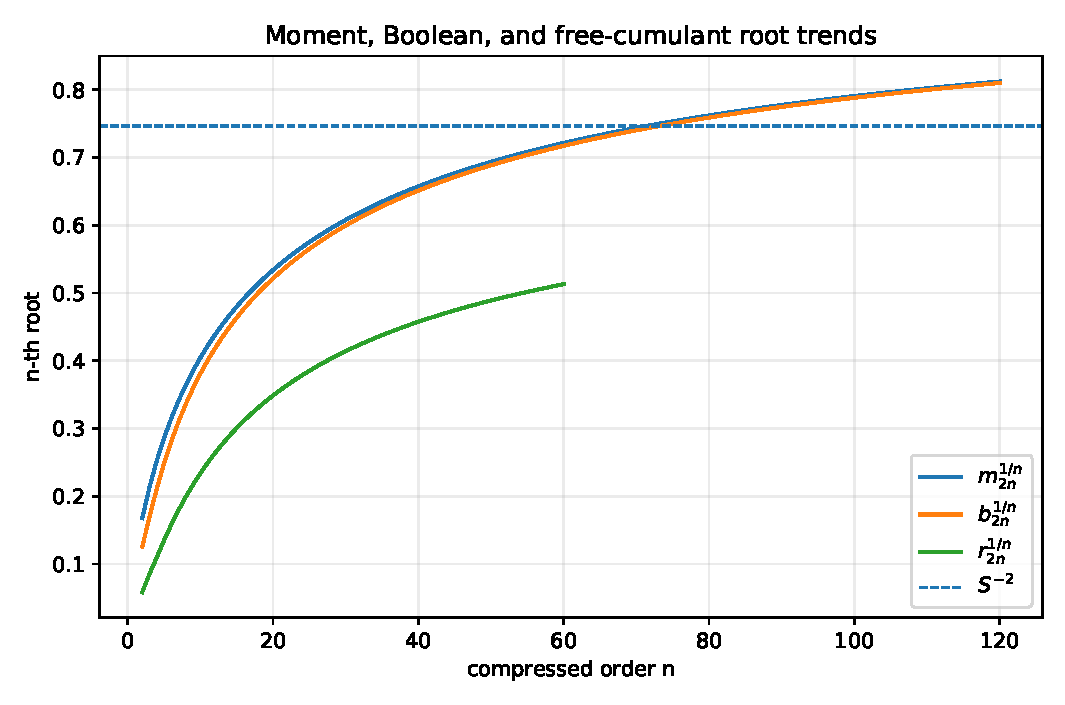
\includegraphics[width=0.78\textwidth]{figures/cumulant_root_trends.pdf}
\caption{Root diagnostics. The moment and Boolean roots tend slowly to one, while the free-cumulant roots appear to approach the horizontal value \(S^{-2}\). The observed convergence is too slow to be treated as proof.}
\label{fig:roottrends}
\end{figure}

\subsection{Why Lambert--\texorpdfstring{\(W\)}{W} should reappear}
The repository's endpoint analysis expresses the saddle location and the flat decay of \(\Up(1-x)\) through Lambert--\(W\)-type scales. Moments
\[
m_{2n}=2\int_0^1x^{2n}\Up(x)\,dx
\]
are therefore controlled by a moving endpoint saddle whose distance from one is itself described by nested logarithms and Lambert--\(W\). The Boolean transform \(1-A^{-1}\) preserves the endpoint location but changes its amplitude. The free transform additionally rescales the singular location by \(\Psi(1)=S^2\). A full proof of Conjectures~\ref{conj:booleanratio} and \ref{conj:freeradius} should combine:
\begin{enumerate}[label=(\alph*)]
\item the existing all-orders endpoint expansion for \(\Up\);
\item a uniform saddle-point estimate for \(m_{2n-k}/m_{2n}\) when \(k\) ranges from fixed to mesoscopic scales;
\item a defective-renewal theorem for the Boolean coefficients;
\item singular inversion of \(\Psi(t)=tA(t)^2\) in a slit complex neighborhood of \(t=1\).
\end{enumerate}
This is a concrete route by which Lambert--\(W\) enters noncommutative cumulant asymptotics rather than merely the original density.

\section{Cyclotomic and \texorpdfstring{\(q\)}{q}-integer structure}
\subsection{Normalized classical cumulants live in a \texorpdfstring{\(q\)}{q}-integer ring}
Let
\[
[m]_s:=\frac{1-s^m}{1-s}=1+s+\cdots+s^{m-1}.
\]
After variance normalization, \eqref{eq:stdclassical} can be written
\begin{equation}\label{eq:lambdakrational}
\lambda_{2m}(s)=
\frac{3^m2^{2m}B_{2m}}{2m}\frac{(1-s)^{m-1}}{[m]_s}.
\end{equation}
Thus every denominator is cyclotomic: its complex zeros are roots of unity other than one.

\begin{proposition}[Cyclotomic denominator control]\label{prop:cyclotomic}
For fixed \(n\), the variance-normalized moment, free cumulant \(c_{2n}(s)\), and Boolean cumulant belong to
\begin{equation}\label{eq:qring}
\mathbb Q\bigl[s,[2]_s^{-1},[3]_s^{-1},\ldots,[n]_s^{-1}\bigr].
\end{equation}
In particular, they have no pole on the positive real interval \(0<s<1\).
\end{proposition}
\begin{proof}
The normalized classical cumulants of orders at most \(2n\) belong to the ring \eqref{eq:qring} by \eqref{eq:lambdakrational}. Moments, free cumulants, and Boolean cumulants of order \(2n\) are universal polynomials with rational or integer coefficients in those classical cumulants. The ring is closed under these operations. Since \([m]_s>0\) on \((0,1)\), no positive pole occurs.
\end{proof}

The explicit denominators in Proposition~\ref{prop:qfree} and Appendix~\ref{app:qformulas} are cancellations and factorizations of products of \([m]_s\). For example,
\[
[2]_s=1+s,
\quad [3]_s=1+s+s^2,
\quad [4]_s=(1+s)(1+s^2),
\]
while \(1-s+s^2\) is the sixth cyclotomic polynomial and arises after cancellation among the \([m]_s\).

\subsection{A \texorpdfstring{\(q\)}{q}-binomial expansion problem}
The ring statement is structural but not yet canonical. It suggests looking for formulas of the form
\begin{equation}\label{eq:qbinomialdesired}
c_{2n}(s)=\sum_{\lambda\vdash n-1}
\frac{P_{n,\lambda}(s)}{\prod_j[j]_s^{\lambda_j}},
\end{equation}
where \(P_{n,\lambda}\) has a sign, positivity, or palindromicity property and the sum is indexed by connected partition types. Such a formula would merge three existing structures:
\begin{enumerate}[label=(\roman*)]
\item Bernoulli numbers from the uniform summands;
\item noncrossing/connected partitions from free cumulants;
\item \(q\)-integers and Gaussian-binomial identities from the geometric weights.
\end{enumerate}

\begin{conjecture}[Cyclotomic numerator regularity]\label{conj:cyclotomicnumerator}
After multiplication by a minimal product of \([j]_s\), the numerator of \(c_{2n}(s)\) has a finite decomposition into reciprocal or anti-reciprocal pieces indexed by connected partition block profiles. The decomposition, rather than the fully expanded numerator, has integer coefficients of controlled sign.
\end{conjecture}
The raw numerator of \(c_{12}\) already has large positive coefficients and a small negative constant term, suggesting that any positivity statement must occur before full cancellation.

\section{Further frontier directions}
\subsection{A proof program for Jacobi-increment positivity}
Conjecture~\ref{conj:jacobiincrements} is especially promising because it explains a striking combination of facts: the dyadic up-law appears to have positive even free cumulants, its Jacobi parameters appear monotone, yet it is not freely infinitely divisible. A proof program could proceed as follows.

First, express moments as weighted Dyck paths with a down-step from height \(j\) weighted by \(\beta_j\). Second, express free cumulants by a connectedness constraint on those paths, using Lehner's irreducible-lattice-path expansion. Third, mark each occurrence of \(\beta_j\) as \(\beta_1+\Delta_1+\cdots+\Delta_{j-1}\). The difficulty is to construct a cancellation-free involution or direct class whose weight is the resulting monomial. The monomial counts
\[
1,3,10,35,120,410,1400
\]
suggest a rapidly growing connected path family and may help identify the correct combinatorial class.

\subsection{Determining the full free-divisibility region}
The leading-Hankel thresholds in Table~\ref{tab:hankelthresholds} appear to stabilize near \(q\approx0.6187\), tantalizingly close to but not exactly the inverse golden ratio. This numerical observation should not be overinterpreted. Leading principal minors are only part of conditional positive definiteness; nonprincipal minors and other test vectors can fail later. A robust investigation should:
\begin{enumerate}[label=(\alph*)]
\item compute all principal and selected nonprincipal minors to increasing order;
\item formulate the conditional free L\'evy measure, if one exists, from the free cumulants;
\item use the reciprocal Cauchy transform to test the Pick/Nevanlinna criterion for free infinite divisibility;
\item compare the analytic continuation threshold with the Gaussian limit \(q\uparrow1\).
\end{enumerate}
An exact proof of a phase transition would likely need analytic control of the Voiculescu transform, not only moment matrices.

\subsection{Free and Boolean transforms of the inverse function}
Formula \eqref{eq:inverseFfree} gives finite integral invariants of \(F^{-1}\), but it does not yet exploit the all-orders inverse endpoint expansion. One can insert the repository's Lambert--\(W\) expansion of \(F^{-1}(u)\) near zero into \eqref{eq:inverseFmoment} and then apply the finite cumulant transforms. This should yield asymptotic expansions for large-order free and Boolean cumulants in terms of the same Bell-polynomial coefficient packages already used for the inverse Fabius function.

A particularly concrete target is an expansion
\begin{equation}\label{eq:rnasymtarget}
r_{2n}=S^{-2n}\exp\!\left[-\Theta\!\left(\frac{n}{W(n)}\right)\right]
\times\bigl(\text{explicit Lambert--\(W\) series}\bigr),
\end{equation}
with the correct scale and prefactor to be determined. Equation \eqref{eq:rnasymtarget} is a research template, not a claimed asymptotic formula.

\subsection{Legendre and Jacobi error transport}
Proposition~\ref{prop:Legendretransform} is triangular. If a numerical Legendre expansion has coefficient errors \(\delta a_{2k}\), then
\[
\delta m_{2n}=\sum_{k=0}^n
\frac{2(2n)!}{(2n-2k)!!(2n+2k+1)!!}\delta a_{2k}.
\]
Combining this with the Jacobian of the moment-to-free-cumulant map gives certified error bars for \(r_{2n}\). Conversely, the exact rational dyadic cumulants provide nonlinear moment constraints that can detect hidden loss of precision in high-order Legendre or Jacobi computations. This is a practical bridge between the repository's representation volumes and the exact arithmetic developed here.

\subsection{Beyond the dyadic base}
For \(|q|<1\), symmetry reduces negative \(q\) to positive \(|q|\), so Theorem~\ref{thm:qnotFID} immediately extends to
\[
0<|q|<0.523498599534498\ldots.
\]
For \(|q|>1\), the infinite series \eqref{eq:Yq} diverges, but finite products can be renormalized by reversing the weights:
\[
q^{-N}Y_q^{(N)}=\sum_{j=0}^{N-1}q^{-j}U_{N-j}.
\]
This converges to a geometric-uniform law with parameter \(1/|q|\). Thus the values \(q=\pm2,\pm4\) are naturally dual to \(q=\pm1/2,\pm1/4\) after finite-level reversal. It would be useful to reformulate the repository's \(q\leftrightarrow q^{-1}\) identities directly at the level of classical, free, and Boolean cumulants.

\subsection{Arithmetic questions}
At \(q=1/2\), every moment and cumulant is rational. Their denominators mix Bernoulli denominators, Mersenne-type factors \(4^m-1\), and partition-transform denominators. Possible arithmetic projects include:
\begin{enumerate}[label=(\roman*)]
\item sharp \(p\)-adic valuations of \(r_{2n}\) and \(b_{2n}\);
\item congruences inherited from von Staudt--Clausen and Kummer congruences for Bernoulli numbers;
\item integrality after multiplication by a canonical product of \((4^j-1)\) and factorial factors;
\item denominator stabilization under finite-level Richardson extraction.
\end{enumerate}
The exact positivity through \(r_{120}\) supplies a substantial initial data set for such experiments.

\subsection{Formal verification}
The central non-free-infinite-divisibility proof is well suited to formalization. Its analytic input can be isolated as the standard theorem ``free infinite divisibility implies conditional positive definiteness of free cumulants.'' The remaining proof is finite:
\begin{enumerate}[label=(\arabic*)]
\item derive the first six even moments from the dyadic cumulant recurrence;
\item derive \(r_2,\ldots,r_{12}\) from noncrossing recurrences;
\item normalize by variance;
\item evaluate the rational quadratic form \eqref{eq:negativeQ}.
\end{enumerate}
This would make a compact Lean extension of the repository's current formalized core. The degree-thirty \(q\)-family theorem is also formalizable, but requires a certified Sturm or polynomial-root library.

\section{Conclusions}
The noncommutative cumulant viewpoint reveals a new set of structures hidden inside the familiar sinc product. The up-law has positive low- and medium-order free cumulants but fails the global Hankel positivity required for free infinite divisibility. This failure is exact, rational, and robust across a nontrivial interval of geometric parameters. Boolean cumulants behave more regularly: Jacobi coefficient stripping proves positivity at every order and identifies them with an associated moment sequence.

The strongest conceptual bridge is that the same finite set of moments simultaneously admits four descriptions:
\[
\begin{array}{c}
\text{Bernoulli numbers and Bell polynomials}\\
\updownarrow\\
\text{infinite or finite sinc products and Thue--Morse splines}\\
\updownarrow\\
\text{inverse-Fabius integrals and Legendre coefficients}\\
\updownarrow\\
\text{free and Boolean cumulants and Jacobi stripping}.
\end{array}
\]
The transformations between these descriptions are finite and exact at each order. This makes the new layer compatible with the repository's existing \(q\)-binomial acceleration, spectral representations, and Lambert--\(W\) asymptotics rather than parallel to them.

The principal open goals are now sharply stated: prove all-order Jacobi-increment positivity, determine the free-divisibility phase diagram of \(Y_q\), and transfer the endpoint Lambert--\(W\) expansion through the Boolean reciprocal and free compositional transforms. Each problem has a concrete algebraic or analytic entry point and a reproducible computational base.

\section{Reproducibility guide}
\label{sec:repro}
The archive contains \texttt{numerical\_experiments.py}. It requires Python 3 together with SymPy, mpmath, and Matplotlib. From the report directory, run
\begin{lstlisting}[language=bash,basicstyle=\ttfamily\small,frame=single]
python3 numerical_experiments.py \
  --output-dir results --figure-dir figures
\end{lstlisting}
The default calculation performs:
\begin{enumerate}[label=(\arabic*)]
\item exact rational dyadic cumulants through \(r_{120}\);
\item the determinant and polynomial-vector certificates;
\item exact symbolic \(c_2,\ldots,c_{12}\), the degree-thirty numerator, root isolation, and Sturm counts;
\item high-precision leading-Hankel thresholds through block size ten;
\item the Jacobi-increment expansion through \(r_{16}\);
\item finite-level \(Q=4^{-N}\) polynomials through order twelve;
\item endpoint moments through \(m_{400}\), Boolean ratios, and figures.
\end{enumerate}
All exact claims are checked with rational or integer arithmetic. Decimal values are printed only after the exact calculation. The generated files under \texttt{results/} include CSV tables and plain-text certificates; figures are available as both PDF and PNG.

\appendix
\section{Explicit normalized \texorpdfstring{\(q\)}{q}-family formulas}\label{app:qformulas}
Put \(s=q^2\). In addition to Proposition~\ref{prop:qfree},
\begin{align}
D_{10}(s)&:=(1+s)^2(1+s^2)(1+s+s^2)(1+s+s^2+s^3+s^4),\nonumber\\
c_{10}(s)&=\frac{2P_{10}(s)}{385D_{10}(s)}.\label{eq:c10full}
\end{align}
where
\begin{align*}
P_{10}(s)={}&2437711s^{10}+646150s^9+757701s^8+780549s^7+782870s^6\\
&+159568s^5+136730s^4+25179s^3+2331s^2+10s+1.
\end{align*}
Also
\begin{align}
D_{12}(s)&:=(1+s)^3(1+s^2)(1-s+s^2)(1+s+s^2)^2\nonumber\\
&\qquad\times(1+s+s^2+s^3+s^4),\nonumber\\
c_{12}(s)&=\frac{2P_{12}(s)}{875875D_{12}(s)}.\label{eq:c12full}
\end{align}
where
\begin{align*}
P_{12}(s)={}&239971210481s^{15}+79887931849s^{14}+98139745702s^{13}
+106474515277s^{12}\\
&+123041556053s^{11}+114309825775s^{10}+52750980414s^9
+35665790305s^8\\
&+27408293365s^7+10846922526s^6+2506486435s^5
+1249569737s^4\\
&+82945993s^3+5673358s^2+3421s-691.
\end{align*}
These formulas specialize at \(s=1/4\) to the normalized dyadic cumulants in Section~4 and at \(s=1\) to the connected-pairing numbers \(248\) and \(2830\).

\section{The degree-thirty Sturm polynomial}\label{app:P30}
Define
\[
P_{30}(s)=\sum_{j=0}^{30}p_js^j.
\]
The coefficients are as follows.
\begin{longtable}{r@{\hspace{2em}}r}
\caption{Coefficients of the determinant numerator \(P_{30}\).}\label{tab:P30coeffs}\\
\toprule
\(j\)&\(p_j\)\\
\midrule
\endfirsthead
\toprule
\(j\)&\(p_j\)\\
\midrule
\endhead
0 & -1 \\
1 & 236797 \\
2 & 154644128 \\
3 & -32161726341 \\
4 & -309530241402 \\
5 & -4962354733999 \\
6 & -25423927396444 \\
7 & -174414460271621 \\
8 & 500704487135269 \\
9 & -1567422948953118 \\
10 & 6462787608357749 \\
11 & 17451160220542367 \\
12 & 47450105349899789 \\
13 & -3112870344293064 \\
14 & 111335265126207640 \\
15 & 260832096100041918 \\
16 & 710585546823441352 \\
17 & 948703157726602056 \\
18 & 944899121577446453 \\
19 & 2149494971059201511 \\
20 & 3586241741057425853 \\
21 & 2006573378166739986 \\
22 & 4423316345984162365 \\
23 & 2656469118337756915 \\
24 & 5387333540324201540 \\
25 & 4570485884957325545 \\
26 & 6277464174324435942 \\
27 & 3802457057684963283 \\
28 & 3106555208559680768 \\
29 & 1365452791577583829 \\
30 & 588031288239582935 \\
\bottomrule
\end{longtable}

The three positive roots are isolated in the rational intervals
\begin{align*}
\frac{6261}{1486660088}&<s_1<\frac{7013}{1665220763},\\
\frac{17338229}{3019459543}&<s_2<\frac{18557046}{3231717013},\\
\frac{385546279}{1406842461}&<s_3<\frac{219810848}{802080713}.
\end{align*}
Numerically,
\begin{align*}
s_1&=0.000004211453613733039418535107394599646153802598\ldots,\\
s_2&=0.005742163043778858179021510344163665436168765139\ldots,\\
s_3&=0.274050783714581103197636083256401808258849748968\ldots.
\end{align*}
An exact Sturm sequence gives three roots in \((0,1)\), no root in \((1/11,s_3^-)\), exactly one in the displayed interval for \(s_3\), and none between its right endpoint and \(1\).


\section{Additional finite-level polynomials}
For reference, the order-ten and order-twelve free-cumulant polynomials are
{\small
\begin{align*}
r_{10}^{(N)}={}&-\frac{2(Q-1)}{23062937695875}
\bigl(930453829171Q^4-628330001950Q^3\\
&\hspace{8em}+149236761408Q^2-14655524050Q+519975421\bigr),\\
r_{12}^{(N)}={}&\frac{2(Q-1)}{214857210441983484375}
\bigl(32015207756442935833Q^5\\
&-24643616781732391817Q^4+7141155293332868434Q^3\\
&-976484255895326266Q^2+64569346306285733Q-1693269622691917\bigr).
\end{align*}}
The order-eight through order-twelve Boolean polynomials are
{\small
\begin{align*}
b_8^{(N)}={}&\frac{4(Q-1)}{3415820625}
\bigl(42029857Q^3-39615618Q^2+13585593Q-1711432\bigr),\\
b_{10}^{(N)}={}&-\frac{4(Q-1)}{115314688479375}
\bigl(3485827553819Q^4-3640877184125Q^3\\
&\hspace{8em}+1538558237937Q^2-317835338375Q+27389330744\bigr),\\
b_{12}^{(N)}={}&\frac{4(Q-1)}{214857210441983484375}
\bigl(22663789837192645279Q^5\\
&-24954751286859145796Q^4+11665865760722459242Q^3\\
&-2968584330536746108Q^2+419917784310690479Q-26668720414063096\bigr).
\end{align*}}
Every displayed expression has degree equal to its compressed order.

\section{A compact proof certificate for the dyadic theorem}
A verifier need only check the following data:
\begin{align*}
r_2&=\frac19,&
r_4&=\frac7{2025},&
r_6&=\frac{562}{893025},\\
r_8&=\frac{55603}{379535625},&
r_{10}&=\frac{148564406}{3294705385125},&
r_{12}&=\frac{3386539245383834}{214857210441983484375}.
\end{align*}
After multiplying \(r_{2n}\) by \(9^n\), form \(H\) in \eqref{eq:Hmatrix}. Then
\[
(3,-4,1)H(3,-4,1)^\top
=-\frac{108624693817191}{404291747234375}<0.
\]
This single rational inequality, together with conditional positive definiteness of free cumulants for freely infinitely divisible laws, proves Theorem~\ref{thm:upnotFID}.

\begin{thebibliography}{99}
\bibitem{ReshetnikovRepo}
V. Reshetnikov,
\emph{ProveIt: Analysis/FabiusFunction documentation corpus},
GitHub repository,
\url{https://github.com/VladimirReshetnikov/ProveIt/tree/main/Analysis/FabiusFunction/docs}.

\bibitem{ReshetnikovFrontiers}
V. Reshetnikov,
\emph{Semi-formalized research frontiers: canonical source, manifest, and draft structure},
\url{https://github.com/VladimirReshetnikov/ProveIt/tree/main/Analysis/FabiusFunction/docs/semi-formalized-research-frontiers}.

\bibitem{Rvachev}
V. L. Rvachev,
Compactly supported solutions of functional-differential equations and atomic functions,
classical papers and monographs cited in the repository corpus.

\bibitem{Fabius}
J. Fabius,
A probabilistic example of a nowhere analytic \(C^\infty\) function,
\emph{Z. Wahrscheinlichkeitstheorie verw. Gebiete} \textbf{5} (1966), 173--174.

\bibitem{Speicher1994}
R. Speicher,
Multiplicative functions on the lattice of noncrossing partitions and free convolution,
\emph{Math. Ann.} \textbf{298} (1994), 611--628.

\bibitem{NicaSpeicher}
A. Nica and R. Speicher,
\emph{Lectures on the Combinatorics of Free Probability},
London Mathematical Society Lecture Note Series 335, Cambridge University Press, 2006.

\bibitem{BercoviciVoiculescu}
H. Bercovici and D. Voiculescu,
Free convolution of measures with unbounded support,
\emph{Indiana Univ. Math. J.} \textbf{42} (1993), 733--773.

\bibitem{ArizmendiHasebeSakuma}
O. Arizmendi, T. Hasebe, and N. Sakuma,
On the Law of Free Subordinators,
\emph{ALEA Lat. Am. J. Probab. Math. Stat.} \textbf{10} (2013), 271--291.
Theorem~2.3 records the equivalence between free infinite divisibility and conditional positive definiteness of free cumulants for compactly supported laws.

\bibitem{LehnerConnected}
F. Lehner,
Free cumulants and enumeration of connected partitions,
\emph{European J. Combin.} \textbf{23} (2002), 1025--1031;
\url{https://arxiv.org/abs/math/0110030}.

\bibitem{LehnerLattice}
F. Lehner,
Cumulants, lattice paths, and orthogonal polynomials,
\emph{Discrete Math. Theor. Comput. Sci. Proc.} (2003);
\url{https://arxiv.org/abs/math/0110031}.

\bibitem{SpeicherWoroudi}
R. Speicher and R. Woroudi,
Boolean convolution,
in \emph{Free Probability Theory}, Fields Institute Communications 12,
American Mathematical Society, 1997, 267--279.

\bibitem{HasebeSakumaNormal}
T. Hasebe and N. Sakuma,
The normal distribution is freely infinitely divisible,
\emph{Comm. Math. Phys.} \textbf{349} (2017), 179--200;
\url{https://arxiv.org/abs/1305.0924}.

\bibitem{Flajolet}
P. Flajolet,
Combinatorial aspects of continued fractions,
\emph{Discrete Math.} \textbf{32} (1980), 125--161.

\bibitem{GasperRahman}
G. Gasper and M. Rahman,
\emph{Basic Hypergeometric Series}, 2nd ed.,
Encyclopedia of Mathematics and its Applications 96,
Cambridge University Press, 2004.

\bibitem{Comtet}
L. Comtet,
\emph{Advanced Combinatorics: The Art of Finite and Infinite Expansions},
D. Reidel, 1974.
\end{thebibliography}

\end{document}
